\documentclass{article}
\usepackage{times}
\usepackage{graphicx}
\usepackage{subfigure} 
\usepackage{hyperref}
\usepackage{amsmath}
\usepackage{amssymb}
\begin{document}
	%Tom
	\section{Data search}
	
	%Ghassen
	\section{LM ARIMA}
	
	%Vlad
	\section{Kelly trading strategy}
	
The primary means through which our analysis is replicable, falsifiable, and quantitatively assessable is by assessing investment performance. Raw accuracy of prediction does not present a fair evaluation of our algorithm, since we need to consider inherent difficulties with predicting the market. In other words, if we make a significant amount of money (e.g. compare the mean returns to S\&P alpha), then there is some inefficiency in the market that our algorithm correctly enables us to take advantage of.

We will use strong simplifying assumptions: we can trade stock at any volume at the EOD price instantaneously without affecting the market. To some extent these assumptions can hold assuming we create a portfolio of commodities, which artificially lowers market presence in individual ones.

That said, we need to convert our model into an actual strategy. Consider the random variable for the EOD price of a commodity $p_i$ for day $i$. Our LM and ARIMA Models provide for $X = \log\frac{p_{i+1}-p_i}{p_i}$ and $X'=X|p_{<i},\text{news}$ an estimate $\mu=\mathbb{E}(X')$ and $\sigma^2=\mathbb{V}(X')$.

The Kelly Criterion (in the continuous case) gives the optimal betting proportion (given an investment, you should only bet a part of it if you're unsure and leverage it if you aren't). This doesn't make any stronger assumptions about the returns (which should be normal about our prediction) than the models do. Then, each day, we need to buy or short sell $\text{sgn }\mu\cdot\frac{\left|\mu\right|-r}{\sigma^2}$ proportion of our investment, where we sell or buy back all our holdings the next day. We purchase leverage at the risk-free rate $r$, so we only invest when we can earn over that much.

Source: http://wwwf.imperial.ac.uk/~mdavis/docs/DavisLleoKellyChapter.pdf

Here's an example run. The purple line is a trading strategy with $\mu\sim\text{Unif}(-5,5)$ and the tan line has $\mu\sim\text{Unif}(-1,1)$. Both have $\sigma^2\sim\text{Unif}(0.25,10)$. The following has $r=0$:

\begin{center}
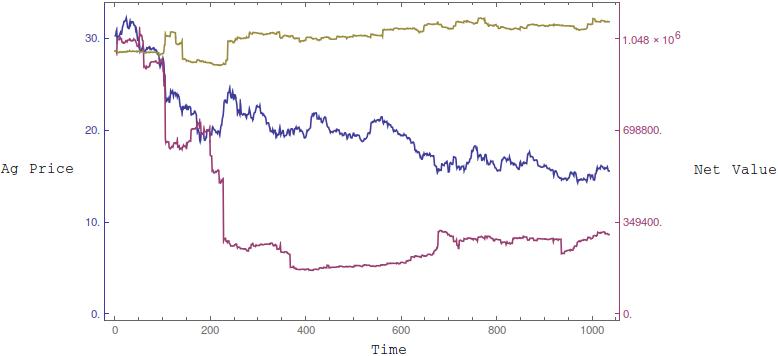
\includegraphics[scale=0.5]{../KellyRun-Random.png}
\end{center}

Notice when we're really confident we tend to leverage {\em a lot}. We might want to have a minimum uncertainty bound, maybe based on stock volatility.

	%Daway
	\section{Clustering}
\end{document}
